\documentclass[conference]{IEEEtran}
\IEEEoverridecommandlockouts

% List of packages used 
\usepackage{cite}
\usepackage{mathtools}
\usepackage{listings}
\usepackage{amsmath,amssymb,amsfonts}
\usepackage[hidelinks]{hyperref}
\usepackage{algorithmic}
\usepackage{graphicx}
\usepackage[]{algorithm2e}
\usepackage{algpseudocode}
\usepackage{textcomp}
\usepackage{xcolor}
\def\BibTeX{{\rm B\kern-.05em{\sc i\kern-.025em b}\kern-.08em
    T\kern-.1667em\lower.7ex\hbox{E}\kern-.125emX}}

% -- Document Starts Here -- 
\begin{document}
\title{\huge{Heuristic Algorithms for Optimization}\\{AI2101 - Group 8}}


% Authors of the document 
\author{\IEEEauthorblockN{1\textsuperscript{st} Member : K.N Vardhan}
\IEEEauthorblockA{\textit{Mathematics and Computing} \\
MA20BTECH11006 \\
ma20btech11006@iith.ac.in}

\and

\IEEEauthorblockN{2\textsuperscript{nd} Member : Tata Sai Manoj}
\IEEEauthorblockA{\textit{Mathematics and Computing} \\
MA20BTECH11018 \\
ma20btech11018@iith.ac.in}

\and

\IEEEauthorblockN{3\textsuperscript{rd} Member : VKS Deepak Reddy}
\IEEEauthorblockA{\textit{Mathematics and Computing} \\
MA20BTECH11019\\
ma20btech11019@iith.ac.in}}

\maketitle

% Abstract
\begin{abstract}
This paper covers three heuristic algorithms in optimization, consisting of the Travelling Salesman Problem using a heuristic approach (Simulated Annealing), Tabu-Search heuristic and Ant Colony Optimization (ACO) heuristic for the Knapsack Problem. 
\end{abstract}

% Introduction 
\section{\textbf{Introduction}}
A heuristic algorithm is a procedure that produces near-optimal solutions to an optimization problem. 
However, such solutions are achieved by trading optimality, completeness, accuracy, or precision for speed.

% Sai Manoj Presentation - TSP 

\section{\textbf{The Travelling Salesman Problem}}

\subsection{Introduction to the problem }
The Travelling Salesman Problem (also denoted by $\textbf{TSP}$ (or) $\textbf{TSP-OPT}$) is a well-known optimization problem. However, the $\textbf{TSP-OPT}$ is NP-hard. We do not know an efficient way to verify a solution for $\textbf{TSP-OPT}$, so we cannot say that it is NP-complete. 

\subsection{Problem Description}
The problem can be simply stated as follows :  
For a given list of cities and the distances between pairs of cities, we have to find the shortest possible route that goes through each city exactly once. 
A naive approach would be to calculate the distance for each possible route, which would involve calculating distances for $n!$ routes. However, this is extremely inefficient, and the time required for computation blows up. 

\subsection{Formulation of the problem}

The $\textbf{TSP}$ can be formulated as an integer linear programming problem. Here, $N$ represents the number of cities and $obj_{ij}$ represents the cost of travelling from city $i$ to city $j$. 
The decision variables are $x_{ij}$, which can take a value of $0$ or $1$, depending on the existence of an edge between city $i$ and city $j$. 

minimize \hspace*{10mm}$\Sigma_{i \in n} \Sigma_{j \in n} (obj_{ij}) \times (x_{ij})$ \\
\hspace*{2.5mm} subject to \hspace*{8mm} $\Sigma_{i \in n} x_{ij} = 1$ $\forall j \in N$\\
\hspace*{27 mm} $\Sigma_{j \in n} x_{ij} = 1$ $\forall i \in N$\\
\hspace*{27 mm} $\Sigma_{i \in n} x_{ii} = 0$

\subsection{Why is TSP NP-hard?}
We claim without proof, that any instance of the Travelling Salesman Problem can be reduced to verifying if a graph has a Hamiltonian Cycle. It is well known that this problem is NP-hard. 

\begin{figure}[htp]
\centering
    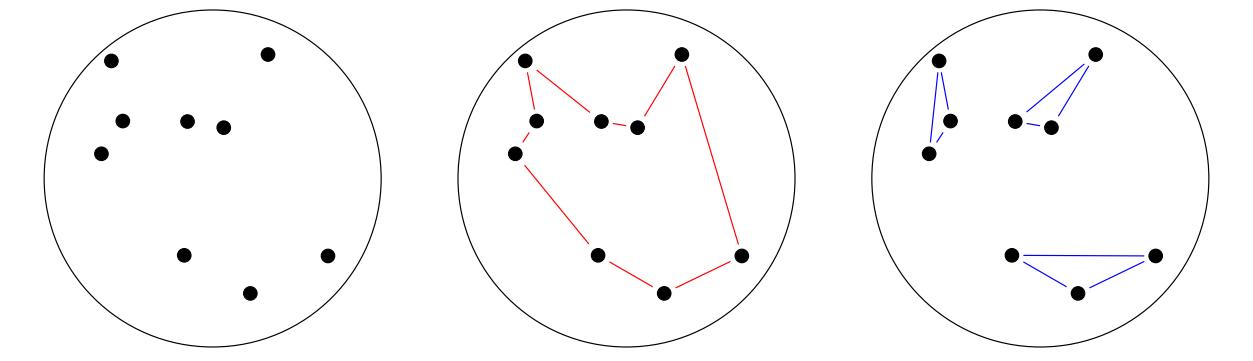
\includegraphics[width=6.5cm]{NPHard.png}
    \caption{Intuition for the NP-hardness of TSP-OPT}
    \label{fig : Intuition for the NP-hardness of TSP-OPT}
\end{figure}

The third diagram satisfies the conditions of the given problem, but it is not "connected". We have to avoid such "local optima" and satisfy the global constraint of staying "connected". 

\section{\textbf{Heuristic Approach : Simulated Annealing}}
The heuristic that we use to find a near-optimal solution for the \textbf{TSP} is Simulated Annealing (\textbf{SA}). The word "annealing" is an analogy to a thermodynamic process in which metal is raised to a high temperature and then gradually decreased to obtain it in a desired state. Similarly, our algorithm starts from a initial solution (say $x$), and keeps generating candidate solutions (say $y_i$) until the stopping criterion for $i$ is reached. 

\subsection{Why this heuristic?}\label{AA}
Simulated Annealing heuristic is only dependent on the following conditions :- 

\begin{itemize}
    \item{The initial solution ($x$)}
    \item{The choice of each candidate solution ($y_i$)}
    \item{The stopping criterion}
\end{itemize}

\subsection{How the algorithm works?}
\begin{itemize}
    \item The \textbf{moving direction} must be determined in a probabilistic way at each step because we do not want to get stuck at a local optimum.
    \item The \textbf{search step} is gradually reduced in size (after every iteration), because the choices we make as we approach the optimal result must be highly optimized. 
\end{itemize}

\subsection{Details of the algorithm }
The following are the steps performed by the algorithm : - 

\begin{enumerate}
    \item Create an initial solution ($x$) by obtaining a random shuffle of the cities. This is our initial route navigating through the cities. 
    \item For every iteration of the algorithm, two of the cities are swapped. This is continued until the stopping criterion is satisfied.
    \item If the overall cost function is reduced, the swap is kept, and a new candidate solution ($y_i$) is generated. 
    \item If the cost function increases, the swap is not $\textbf{rejected}$. The swap may be included with certain probability. 
    \item Now, the temperature is updated after the iteration, slowly "cooling" down (this affects the chances of rejected swaps in the candidate solution).
\end{enumerate}

% Inserting Flowchart
\begin{figure}[htp]
    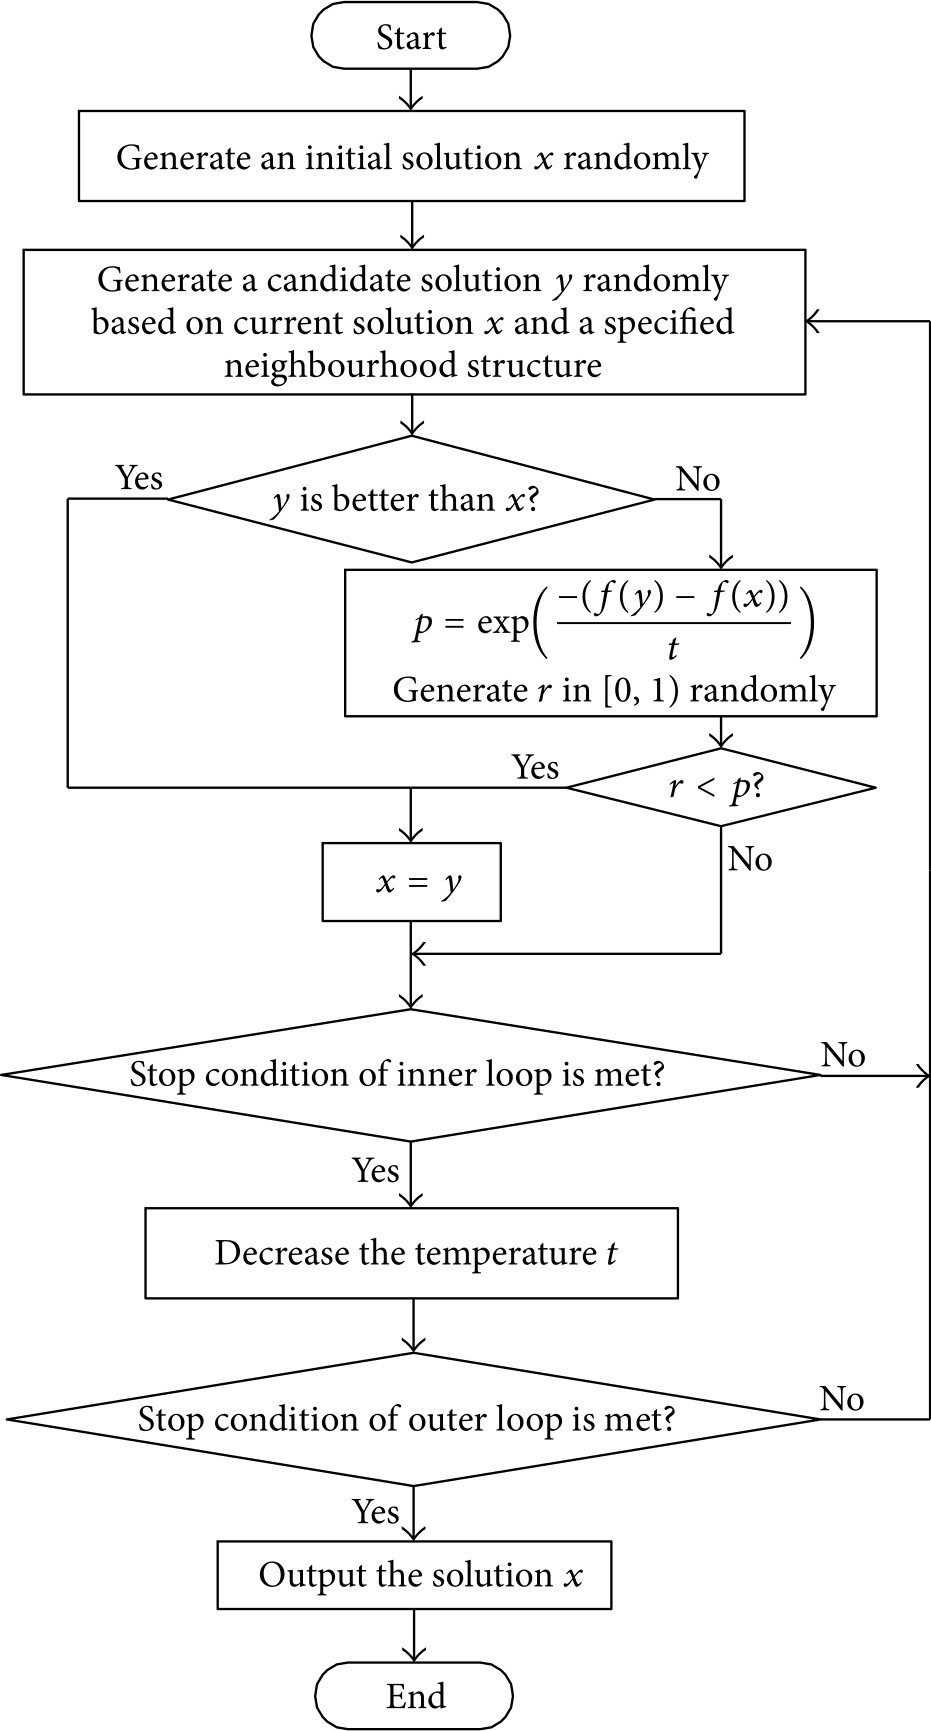
\includegraphics[width=8cm]{SA_flowchart}
    \caption{A general SA algorithm}
    \label{fig : General steps for a Simulated Annealing algorithm}
\end{figure}

\newpage
\subsection{High Level Algorithm Description}
\begin{algorithm}

    \SetKwInput{KwData}{Variables}
    \SetKwInput{KwResult}{Output}
    
    \KwData{Initial Temperature $T_0$, Minimum Temperature $T_{min}$, Maximum number of iterations $K_{max}$, Probability of temperature drop $\rho$, Objective Function ${obj}$}
    \KwResult{Generating the optimal solution}
    
    \begin{itemize}
        \item{Generate an initial solution $x_{0}$}
        \item{$x_{opt} = x_{0}$}
        \item{Compute ${obj}(x_0)$ and ${obj}({opt})$}
        \item{$T_{opt} = T_0$}\\
    \end{itemize}
    
    \While{$T_{opt} > T_0$}
    { 
        $\Delta f$ = $f(x_{curr}) - f(x_{opt})$
        
        \If{$\Delta f < 0$}
        {
            $x_{opt} = x_{curr}$\;
        }
        \EndIf
        \If{$\Delta f >= 0$}
        {
            $\rho$ = $e^{(\frac{\Delta f}{t})}$\;
            \If{rand(0, 1) $\geq \rho$}
            {
                $x_{curr} = x_{new}$\;
            }
            \EndIf
        }
        \EndIf
        $i = i + 1$\;
        $T_{i} = \rho$ $\times$ $T_{i}$
    }
\end{algorithm}

\subsection{Some more possible optimizations}
\begin{itemize}
	 \item{The probability function that is used in the description of the algorithm is the random function, which selects a value between $[0, 1]$. We can use better probabilistic distributions which give a more optimal solution in lesser number of iterations.}
	 \item{The temperature can be updated in multiple different ways (other than the one given in the description). Quadratic cooling, exponential cooling and logarithmic cooling can capture the variation better than linear cooling.}
\end{itemize}

\subsection{Visualization}
The following $\href{https://perrygeo.github.io/sa-tsp-cljs/}{\textbf{link}}$ is an animation of the Travelling Salesman Problem with Simulated Annealing. 

\newpage
\begin{center}
\Large{\textbf{Tabu Search Heuristic}}
\end{center}
\setcounter{section}{0}
\renewcommand*{\theHsection}{chX.\the\value{section}}

\begin{left}
\section{\textbf{Introduction}}
\end{left}

When we are working on convex optimization problems, the local optima is always the
global optima, so the local optimization techniques converge to local optimum but we
get still get the global optima. However, in case of non-convex problems, when we use convex
optimization techniques we might end up with some local optima which is not the global
optima as such a method only permits moving to neighboring solutions that improve the
current objective function value and ends when no improving solutions can be found.
So, we need techniques that can escape from local optima in order to search the
solution space beyond local optima, more extensively and effectively to reach the global
minima.
\vspace{6mm}

\begin{figure}[htp]
\centering
    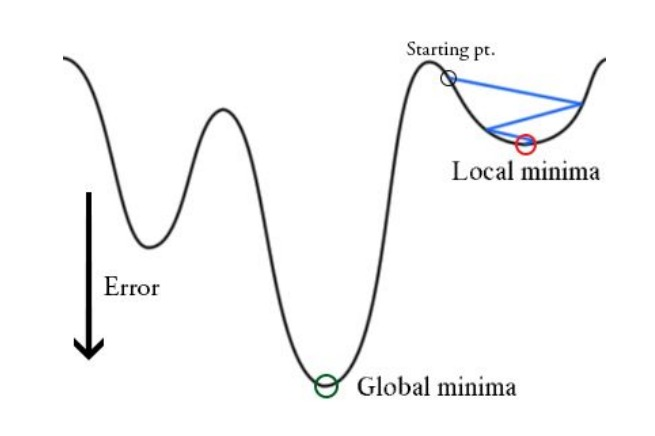
\includegraphics[height = 6cm]{Optima.jpeg}
    \caption{Local Optima and Global Optima}
    \label{fig : Local Optima and Global Optima}
\end{figure}

Also, when solving a real-world problem, finding the optimal global solution in
reasonable amount of time is necessary . However, finding exact solutions is difficult
because resources are constrained, and most of the optimization problems are
complex. Heuristic algorithms can solve this difficulty by offering approximate solutions.
Different Heuristic algorithms are pretty extensive to various applications to solve nonlinear non-convex and combinatorial optimization problems.

Tabu search is one such Heuristic algorithm, which incorporates an iterative, adaptive
memory-based neighborhood-search method. It can used on non-convex problems to
get an approximate globally optimal solution.

\section{\textbf{Understanding Tabu Search}}

Tabu search basically begins in the same way as an ordinary local or neighborhood search, proceeding iteratively from one point (solution) to another until a chosen termination criterion is satisfied.

\subsection{Neighbourhood construction}
Consider $X$ to be the search space, each solution $x$ has an associated neighborhood $N(x)\subset X $, and each solution $x′\in N(x)$ is reached from x by an operation called a move. Tabu search permits moves that deteriorate the current objective function value and selects the moves from a modified neighborhood $N^{*}(x)$, which is the result of maintaining a selective history of the states encountered during the search.

Such construction of the neighborhood reinforce the primary interest of TS, which is to define neighborhoods in dynamic ways that can allow search to move beyond local optima and include simultaneous consideration of multiple types of moves.

\subsection{Recency based memory and Frequency based memory}

The Selective history uses attributive memory, the type of memory records information about solution properties (attributes) that change in moving from one solution to another rather than the solution itself to save space.

There are two types of \textbf{attributive memory}, Recency based memory structures and frequency based memory structures. 
\textbf{Recency based memory structure} keeps track of solutions attributes that have changed during the recent past. Selected attributes that occur in solutions recently visited are labeled tabu-active and these changes of attributes are restricted up to certain iteration (\textbf{Tabu tenure}). This prevents certain solutions from the recent past from belonging to $N^{*}(x)$ and hence from being revisited.

\textbf{Frequency based memory structures} keep track of solution attributes that occur with certain frequency in previous iterations and make such changes in attributes, tabu active. Both of these are short-term memories and encourage \textbf{Diversification} (drive the search into regions dissimilar to those already examined) which is particularly helpful when better solutions can be reached only by crossing barriers or “humps” in the solution space topology.

\textbf{Intensification} (Jump to or initiate a return to regions in the configuration space in which some stored elite solutions lie: these regions can then be searched more thoroughly) strategies require a means for identifying a set of elite solutions as basis for incorporating good attributes into newly created solutions. To store these we need Long term memory structures.
A key element of the adaptive memory framework of tabu search is to create a balance between search intensification and diversification.

Moves or solutions that are part of the \textbf{Aspiration Criteria} (optional) cancel out the Tabu and the move can be made even if it’s in the Tabu List. This can also be used to prevent \textbf{stagnation} in cases where all possible moves are prohibited by the Tabu List.

\newpage
\section{\textbf{Algorithm for Tabu Search}}
\subsection{Steps in the Algorithm}
\textbf{Step 1}:
Start with an initial solution $x = x_{0}$. This can be any solution that fits the criteria for an acceptable solution. And initialize best solution $x_{b} = x_{0}$. 

\textbf{Step 2}:
Generate a set of neighbouring solutions to the current solution $x$ labeled $N(x)$. From this set of solutions, the solutions that are in the Tabu List are removed with the exception of the solutions that fit the Aspiration Criteria. This new set of results is the new $N^{*}(x)$.

\textbf{Step 3}:
Choose the best solution out of $N^{*}(s)$ and label this new solution $x’$. If the solution $x’$ is better than the current best solution, update the current best solution, $x_{b} = x’$. Then, regardless if $x’$ is better than $x$, we update $x$ to be $x’$.

\textbf{Step 4}:
Update the Tabu List $T(x)$ by removing all moves that are expired past the Tabu Tenure and add the new move $x’$ to the Tabu List. Additionally, update the set of solutions that
fit the Aspiration Criteria $A(x)$. If frequency memory is used, then also increment the frequency memory counter with the new solution.

\textbf{Step 5}:
If the Termination Criteria are met, then the search stops or else it will move onto the next iteration. 
Termination Criteria is dependent upon the problem at hand but some possible examples are:

\begin{enumerate}
\item{a max number of iterations}
\item{if the best solution found is better than some threshold}
\end{enumerate}

\vspace{4mm}
\begin{figure}[htp]
\centering
    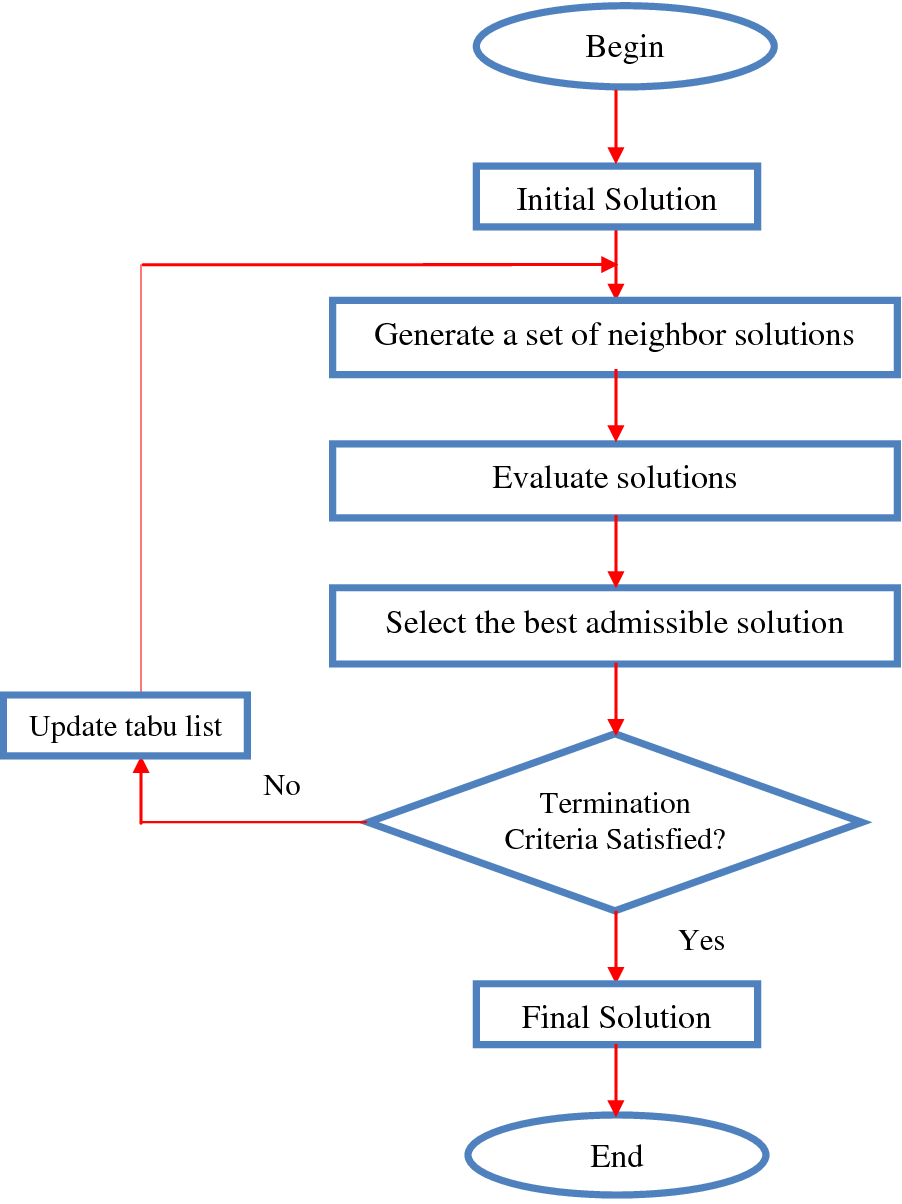
\includegraphics[height = 10cm]{Tabu_Search_Flowchart.png}
    \caption{Tabu Search Flowchart}
    \label{fig : General steps for a Simulated Annealing algorithm}
\end{figure}

\newpage
\subsection{Single Machine Total Weighted Tardiness Problem (SMTWTP)}

Consider a set of $n \in N$ jobs that need to be processed on a single machine that can handle at most one job at a time. Each job $j$ is assigned to a processing time $p_{j} \belongs N \geq 0$ that describes the time that is needed to process job j, a due date $d_{j} \in N \geq 0$ that describes the time point when the processing of job j should have been finished, and a weight $w_{j} \in N \geq 0$ that represents the priority of job $j$.

Given such a set of $n$ jobs, a schedule $\pi$ is a permutation of length $n$, i.e., a bijective
mapping

\begin{center}
$\pi \colon {[1, 2, ..., n]} \to {[1, 2, ..., n]}$
\end{center}

that assigns to each place $i$ in the queue a job $\pi (i)$. For the sake of a clear notation, we represent a permutation $\pi$ as the $n$-tuple $(\pi (1), ..., \pi (n))$. Clearly, a schedule $\pi$ defines a
total order in which the n jobs are processed on a single machine with $\pi (1)$ (respectively
$\pi (n)$) being the first (respectively last) job in $\pi$. 

For a given schedule $\pi$, the completion time $C_j$ of a job $j$ is the time that is needed to complete job $j$ in $\pi$, i.e.,

\begin{center}
    $C_j = \Sigma^{i \leq \pi^{-} (j)}_{i = 1} p_{\pi (i)} $
\end{center}

where $ \pi^{-} (j)$ denotes the position of job $j$ in $\pi$.
The tardiness $T_j$ of a job $j$ is defined as

\begin{center}
    $T_j \coloneqq max{\{C_j - d_j, 0\}}$
\end{center}

Note that the tardiness cannot be negative and thus, it can be seen as a penalty for completing a job after its due date.
Given a set of $n$ jobs, SMTWTP aims to find a schedule of all $n$ jobs that minimizes the weighted tardiness of all jobs, i.e., it aims to minimize the objective function. 

\begin{center}
    $\Sigma^{n}_{j = 1} w_j T_j$
\end{center}

The expression of a schedule $\pi$ is also called the total weighted tardiness of $\pi$. 
In terms of only initially given variables our objective is 
\begin{center}
    $\min (\Sigma^{n}_{j = 1} w_j * max{\{\Sigma^{i \leq \pi^{-}(j)}_{i = 1}} p_{\pi (j)} - d_j, 0\})$
\end{center}

\newpage
\subsection{Pseudocode for Tabu Search Algorithm}
\begin{lstlisting}
TabuSearch()

    START while termination 
        criterion is false
        SET value = BestMove ()
        MAKE best_move
        MAKE best_move tabu
        if value < global_best
            global_best = value
        END if
    END while
END TabuSearch

BestMove()

    START for i less than n
        START for j = i + 1 till n
            swap (sequence[i,j]) 
            value = objective(sequence)
            if tabu[i][j] && 
               value > global_best
                continue
            END if
            if value < best_so_far
                best_so_far = value
                best_move = [i,j]
            END if
        END for
    END for
    return best_so_far
    
END BestMove

\end{lstlisting}

\newpage
\setcounter{section}{0}
\renewcommand*{\theHsection}{chX.\the\value{section}}
\begin{center}
\Large{\textbf{Knapsack Problem}}
\end{center}
\section{\textbf{Introduction}}

A heuristic algorithm sacrifices optimality, accuracy, precision, or completeness for speed to solve a problem faster and more efficiently than standard approaches. When approximate answers are satisfactory but exact solutions are computationally costly, heuristic algorithms are frequently used.

\par
One of the common use of heuristics is to solve the Knapsack problem. The knapsack problem is a problem in combinatorial optimization. Given a set of items, each with a weight and a value, determine the number of each item included in a collection. The total weight is less than or equal to a given limit, and the real value is as significant as possible.

\section{\textbf{Knapsack Problem}}
The heuristic algorithm for this problem used is \textit{Greedy Approximation Algorithm}, which sorts the items based on their value per unit mass and adds the items with the highest $v/w$ (value/weight) as long as there is still space remaining. There exist various kinds of knapsack problems.

\par
Different Knapsack Problems: 0-1 knapsack problem, bounded knapsack problem (BKP), unbounded knapsack problem (UKP).

The knapsack problems are interesting from different perspectives. 
\begin{itemize}
	\item The decision problem form of the knapsack problem is NP-complete. Thus, there is no known algorithm for different test cases, both correct and fast.
	\item There is a pseudo-polynomial time algorithm using dynamic programming.
	\item While the decision problem is NP-complete, the optimization problem is not, and there is no known polynomial algorithm that can tell, given a solution, whether it is optimal
\end{itemize}

In order to obtain the solution of a 0-1 Knapsack problem in a short time period, we use heuristic algorithms. Here, we see the Ant Colony Optimization (ACO) algorithms to provide better performance for solving the 0-1 Knapsack Problem. These algorithms are a class of algorithms inspired by observing the real ants. Real ants can locate the quickest path between their colony and a food source through biological principles.

\subsection {Mathematical formulation}
In the 0-1 knapsack problem, the given elements are:

\begin{center}
    $n$ objects,\\
    $i^{th}$ object has weight $W_i$,\\
    $P_i$ is the profit of $i^{th}$ object,\\
    $M$ as the weight limit of the knapsack.
\end{center}

Our \textit{objective} is to maximize the profit $P_{net}$ under the \textit{constraint} that the total weight $W_{total}$ is at most equal to $M$.

\par
Thus, it can be formulated as
\[Maximize\:\: z= \sum_{i=1}^{n} P_iX_i, \: i = 1,2, \dotso n\]

And the constraint being
\[\sum_{i=1}^{n} W_iX_i \leq M, \: i = 1,2, \dotso n;\quad X_i \in \{0,1\}\]

where $X_i$ is the object variable to include or not in the knapsack.

\subsection{ACO Algorithm}
This is a cooperative evolutionary strategy where numerous generations of artificial ants hunt for suitable solutions. Ants are formed randomly on nodes and migrate stochastically from a starting node to viable adjacent nodes.

%Ants acquire and store information in pheromone trails while searching for possible solutions. While constructing solutions, ants might distribute pheromones online. In addition, during the search process, the pheromone will be evaporated to minimize local convergence and expand the search region. More pheromones are dropped to update the pheromone trail, biasing the search process toward the current best path. 

\par
The proposed algorithms are shown here, including a flowchart as well for better understanding.
\begin{algorithm}
\While {ACO hasn't stopped}
	 {Ants-generation-activity() \\	 Pheromone-evaporation() \\ Daemon-actions()}
\end{algorithm}

Each ant builds a complete solution to the problem in several stages, with an intermediate or partial solution at each step. The ant $k$ develops a new intermediate solution by moving from node $i$ to node $j$ in each step. The solution will is obtained in a specific number of steps. Each ant $k$ analyzes a set of possible expansions from its present node at each step and goes to one of them with a high probability.\par

The three functions Ants\_generation\_activity(), Pheromone\_evaporation(), and Daemon\_actions() do specific actions to build up the optimization.

\begin{enumerate}
	\item \textbf{Ants\_generation\_activity()}\\
	The Ants find solutions starting from a start node and moving to feasible neighbor nodes. During this process, the data collected by the ant will be stored in pheromone trails. The search for neighbor nodes is driven stochastically by an ant-decision rule, that is made up of pheromone and heuristic data.
	\item \textbf{Pheromone\_evaporation()}\\
	Here, we decrease the intensities of pheromone trails over time. The pheromone amount diminishes for all objects, which is represented by evaporation. The quantity of the pheromone rises when an additional quantity is added to all objects, which constitutes the best solution. A higher concentration of the pheromone suggests that ants are more likely to choose the object to search for the optimum solution to the problem.\par
	This process is done to avoid convergence from various ants and to explore more search areas.
	\item \textbf{Daemon\_actions()}\\
	It is optional for ant colony optimization, and they are often used to collect useful global data by depositing additional pheromone.
\end{enumerate}

\newpage
In ACO, the Ant starts from a random start node and successively visits other nodes until all of them are visited. The Ant-decision table for the Ant $k$ doing the activity
\begin{center}
node $i$ to node $j$ is governed by
\[\pi(j) = 
	\begin{dcases}
		\arg\{\max\limits_{i=allowed_{k}(t)}[\tau_{ij}(t)\cdot\eta_{ij}^{\beta}]\} & q \leq q_0 \\
		S & otherwise
	\end{dcases}
\]
\end{center}
where 
\begin{itemize}
\item{$\eta_{ij}$ is the heuristic information and is the set as the highest value of $d_j \\(\eta_{ij} = 1/d_j)$}
\item{$\beta$ is a parameter representing the importance of heuristic information}
\item{$q$ is a random number uniformly distributed in $[0,1]$}
\item{$q_0$ is a pre-specified parameter $(o \leq q_0 \leq 1)$}
\item{$allowed_k(t)$ is the set of all feasible nodes that are not yet visited by $k$}
\item{$t$ is at that particular time}
\item{$S$ is an index of the node selected from $allowed_k(t)$}
\end{itemize}
\par
Here, in finding a feasible solution, Ants perform step-by-step pheromone updates as:
\begin{center}
$\tau_{ij}=\tau_{ij}+\Delta\tau_{ij}$
\end{center}
where $\Delta\tau_{ij}$ is the amount of pheromone deposited from the ant while moving from node $i$ to node $j$. The above step is repeated until all the ants have found a feasible solution.
\par

The intensity of evaporation is controlled by the parameter $\rho$. The quantity of the pheromone on each node is updated at the end of every cycle. The pattern of updation of quantity of pheromone on each object at the end of every cycle is
\begin{center}
    $\tau = \rho\tau$ \quad $\rho \in (0, 1]$
\end{center}
\par
The above algorithm is repeated until the stop criteria are met.
\newpage
Depicting the above algorithm in a flowchart manner.\par

\begin{figure}[htp]
\centering
    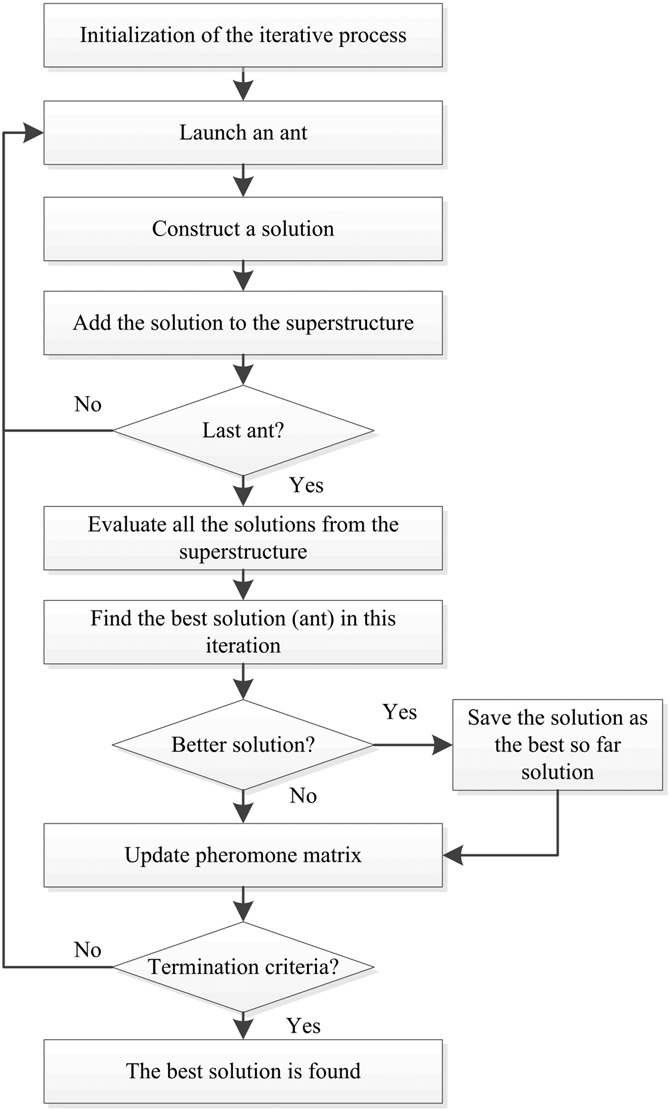
\includegraphics[height = 15cm]{AOC Flowchart.png}
    \caption{Knapsack Flowchart}
    \label{fig : Knapsack Flowchart}
\end{figure}
\newpage
\begin{thebibliography}{9}
\setcounter{section}{0}
\renewcommand*{\theHsection}{chX.\the\value{section}}
\section{Travelling Salesman Problem}

\bibitem{lamport1}
Travelling Salesman Problem \\
\textit{Wikipedia:}
\href{https://en.wikipedia.org/wiki/Travelling_salesman_problem}{TSP Problem}

\bibitem{lamport2}
Simulated Annealing \\
\href{https://www.fourmilab.ch/documents/travelling/anneal/}{TSP with Simulated Annealing}

\bibitem{lamport3}
More on Simulated Annealing \\ \href{https://towardsdatascience.com/how-to-solve-the-traveling-salesman-problem-a-comparative-analysis-39056a916c9f}{Comparison with other methods}

\bibitem{lamport4}
** Credit to Perry Geo for Visualize TSP with Simulated Annealing \\
\href{https://perrygeo.github.io/sa-tsp-cljs/}{Local Host animated TSP}

\section{Knapsack Problem}
\bibitem{lamport5}
Knapsack Problem \\
\textit{Wikipedia:}
\href{https://en.wikipedia.org/wiki/Knapsack_problem}{knapsack problem}

\bibitem{lamport6}
A New Approach for Solving 0-1 Knapsack Problem\\
\textit{2006 IEEE Internation Conference}
\href{https://ieeexplore.ieee.org/document/4274362}{on Systems, Man, and Cybernetics}

\bibitem{lamport7}
The 0-1 Knapsack Problem\\
\textit{Ant Colony \href{https://repozytorium.biblos.pk.edu.pl/redo/resources/30706/file/suwFiles/SchiffK_AntColony.pdf}{Optimization Algorithm}}

\section{Tabu Search Algorithm}

\bibitem{lamport8}
Tabu Search\\
\textit{Wikipedia:}
\href{https://en.wikipedia.org/wiki/Tabu_search}{Tabu Search}

\bibitem{lamport9}
Tabu Search\\
\textit{Research Paper on Tabu Search : }
\href{https://www.uv.es/~rmarti/paper/docs/ts2.pdf}{Fred Glover, Rafael Marti}

\bibitem{lamport10}
Metaheuristic in Optimization : Algorithmic Perspective\\
\href{https://www.uv.es/~rmarti/paper/docs/ts2.pdf}{Metaheuristic in Optimization}

\bibitem{lamport11}
Tabu Search meta-heuristic: Motivations and basic ideas\\
\href{https://web2.qatar.cmu.edu/~gdicaro/15382/additional/tabu-search.pdf}{Heuristic : Tabu Search}

\bibitem{lamport12}
Tabu Search : A comparative study\\
\href{https://www.researchgate.net/publication/221787181_Tabu_Search_A_Comparative_Study}{Comparative Study}

\bibitem{lamport13}
Tabu Search : A brief survey and some real-life applications\\
\href{http://elib.mi.sanu.ac.rs/files/journals/yjor/11/yujorn11p5-17.pdf}{Applications}





\end{thebibliography}
\end{document}

